\documentclass{report}
\usepackage{listings}
\usepackage{hyperref}
\usepackage{tikz}
\usetikzlibrary{shapes.geometric, arrows}
\tikzstyle{process} = [rectangle, minimum width=3cm, minimum height=1cm, text centered, text width=6cm, draw=black]
\tikzstyle{arrow} = [thick,->,>=stealth]

\begin{document}

\title{Tastydoc: a documentation tool for dotty using Tasty files}
\author{Bryan Abate
\\\\\small{Supervised by Aleksander Boruch-Gruszecki}}

\maketitle

\begin{abstract}
The current documentation tool (Dottydoc) relies on compiler internals and low level code. The tool introduced here aims to build a program not dependant on compiler internals but instead use Tasty files which are output when a Scala program is compiled.

It also aims at providing a tool with less bugs, more features and which is more easily maintenable.

For flexibility the output is in Markdown instead of the commonly used HTML.
\end{abstract}

\tableofcontents

\chapter{Introduction}

A documentation tool is a program generating information (often in the form of HTML files) about projects, it usually includes: method signatures, user written documentation, link to other pages, etc.
In Dotty, the current tool for generating Scala project documentation is called Dottydoc. The tool introduced here, called Tastydoc, aims to improve on Dottydoc and replace it.

Tastydoc makes use of TASTy files, they are output when a program is compiled, they contain information about the source code of a program. Tastydoc consumes such files to extract information about the code, that way it is completely independant from the compiler and can be used on its own.
The tool tries to be as close as possible to the structure proposed in Dottydoc so that it can reuses partial portion of its code with minor modificaitions.
As though documentation is often output as HTML files, here we choose to output Markdown files for reasons we detail further in the report.

The tool was developped with a few goals in mind. It should be independant from the compiler, hence the use of TASTy files. It should produce humanly consumable files, hence the choice of Markdown as an output. It should have as much features as Dottydoc and produce a code easily maintenable.

The report is organized in the following structure: First we will talk about the features of the tool, then give a high-level and a low-level architectural description. Dottydoc and Tastydoc will then be compared. We will finally talk about problems encountered during the development, further work and sumarise the project.

\chapter{Features}
We will list here the most important features of Tastydoc. The tool has knowledge of the full signature of entities (classes, defs, vals, etc.), of classes/traits/objects/packages members, of classes constructors, known subclasses of a trait or class, companion and of user written documentation (including @ notations). It offers an easy to use interface (called Representation, see ) to access all these information for anyone willing to write their own documentation tool without worrying to consume TASTy files. The tool relies on TASTy files and is hence independant from the compiler.

The intermediate structure is similar do Dottdoc \texttt{Entity}\footnote{\texttt{dotty/tools/dottydoc/Entity.scala}} which allows for an easy reuse of part of Dottydoc code with minor modifications. Right now, the tool uses some code from Dottydoc for parsing user documentation. But we can think of using it to produce the same HTMl files as does Dottydoc but without relying on compiler internals for example.

Both syntax of user documentation is supported, that is the Wiki and the Markdown syntax. Linking to entities (classes, methods, etc.) is possible inside the user documentation.

Tastdoc is able to link to type defined outside of the current TASTy files (as well as the one inside the file). This is particularly useful for linking to parameters and return types, companions and parents.

The tool produces Markdown documentation files which are easy to modify and read.

\chapter{High-level architectural descriptions}
*** Use TASTy
Data format aimed at serializing compiler information about code,
should be perfect to extract information from.
*** Output Markdown
Can be edited by hand, users can even add their own files;
Easily consumable by other tools - renderable to HTML, PDF;
Can be simply uploaded to Github;
Can be processed by other tools before uploading the documentation;
*** Reuse Dottydoc's intermediate representation
Allows reusing Dottydoc's output;
Dottydoc already has a complex templating mechanism which allows 
attaching blogposts to documentation;

\chapter{Low-level architecture}
Class descriptions etc.

\chapter{Comparison between DottyDoc and TastyDoc}
*** Output/feature differences

\chapter{Problems}
*** No good Markdown library

\chapter{Remaining work}
*** Highlighting type lambdas
*** ...

\chapter{Summary}


\chapter{BELOW IS OLD REPORT, STOP HERE}

\chapter{Introduction}
In dotty the documentation generation tool is called \texttt{dotty-doc}. However the tool is flawed in many ways, these flaws include:
\begin{itemize}
    \item Reliance on compiler internals
    \item Low level and unecessarily complex code which make it hard to maintain
    \item Not maintened and not documented
    \item Not flexible in its output, it outputs HTML/css in a hard to modify way
    \item Malformed type output such as \texttt{[32m"getOffset"[0m}
    \item Classes often show to be extending Object instead of their superclass. Example: \url{https://dotty.epfl.ch/api/scala/Conversion.HTML}
\begin{lstlisting}[language=scala]
abstract class Conversion [ -T, +U ] extends Object with Function1
\end{lstlisting}
    \item Annotations which sould not be display, sometimes are. Example:
    \item Lacks some features, especially:
    \begin{itemize}
        \item No known subclasses
        \item 
    \end{itemize}
\end{itemize}

The tool introduced here aims to address all these issues while providing with a code easy to maintain and easy to adapt to every need.

One major difference with currrent documentation tools is that the output is in Markdown instead of HTML, this has some pros and cons which will be discussed below.

Althought dotty-doc has some problems, the current tool will draw inspiration for some of its architecture which will allow for its parsing code for user documentation (modified to handle this structure and output Markdown) to be reused.

The report will follow the structure described in this introduction and will conclude with problems of the current implementation and further work.

\chapter{Features}

\chapter{Output format}
Before describing the output, we list the reasons, pros and cons of using a Markdown output.

\section{Reasoning behind Markdown}

The major reason to use Markdown instead of HTML is to think of the documentation tool as a pipeline which would look like this:

\begin{center}
    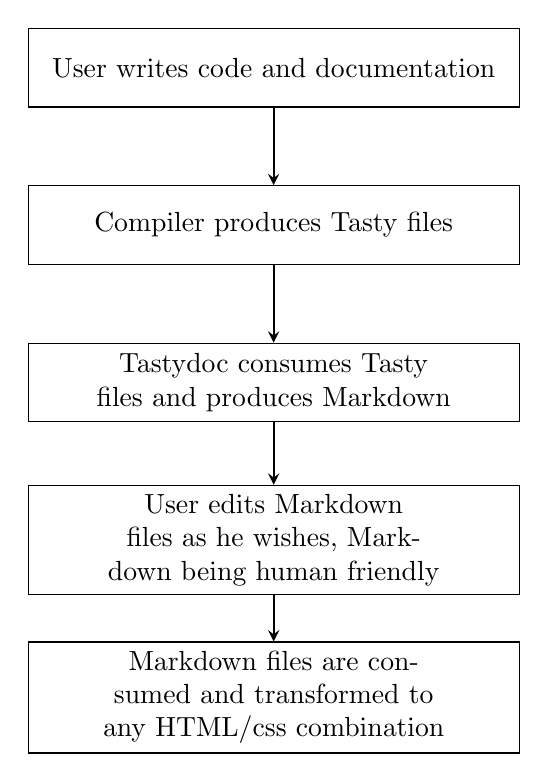
\begin{tikzpicture}[node distance=2cm]
        \node (write) [process] {User writes code and documentation};
        \node (compile) [process, below of=write] {Compiler produces Tasty files};
        \node (tool) [process, below of=compile] {Tastydoc consumes Tasty files and produces Markdown};
        \node (user) [process, below of=tool] {User edits Markdown files as he wishes, Markdown being human friendly};
        \node (HTML) [process, below of=user] {Markdown files are consumed and transformed to any HTML/css combination};
    
        \draw [arrow] (write) -- (compile);
        \draw [arrow] (compile) -- (tool);
        \draw [arrow] (tool) -- (user);
        \draw [arrow] (user) -- (HTML);
    \end{tikzpicture}
\end{center}

With such a pipeline we do not limit the user to use a specific output for the documentation, he can easily remove, add parts, etc. manually and then use an HTML format of his choosing as Markdown only specify the structure not how it should be displayed.

\section{Pros and Cons}
\label{sec:proscons}
Using Markdown as an intermediate output format comes with some pros and cons comparing to an HTML output:
\begin{itemize}
    \item \textbf{Pros:}
    \begin{itemize}
        \item Human readable and editable, meaning part of the documentation can be written manually
        \item Easy to infer the format of the output to extend it manually
        \item Live preview and editing
        \item Only define the structure of the output not how to display it
        \item Easily pipelined to another format (HTML, reStructuredText, etc.)
    \end{itemize}
    \item \textbf{Cons:}
    \begin{itemize}
        \item No Scala (or Java) library available to output markdown with escaping
        \item Markdown fenced code block cannot contain links which forces us to use html code block, hence loose syntax highlight in Markdown and not output "pure" Markdown.
        \item Markdown does not have "division" like \texttt{<div>} in HTML to better structure the output
    \end{itemize}
\end{itemize}

\section{Output structure}
In the following section, we describe how the markdown output is structured.

\subsection{class, object and trait}
Have their own \texttt{.md} file.

\begin{enumerate}
    \item Name (header 1)
    \item Companion object (header 2)
    \item Signature (HTML pre + code)
    \item User documentation
    \item Annotations (header 2)
    \item Known subclasses (header 2)
    \item Constructors (header 2)
    \begin{enumerate}
        \item Name + paremeters (HTML pre + code)
        \item User documentation
    \end{enumerate}
    \item Members (header 2) (In order: Abstract Type Members, Concrete Type Members, Abstract Value Members, Concrete Value Members)
    \begin{enumerate}
        \item Follows structure described in \autoref{sec:signatureSec}
    \end{enumerate}
\end{enumerate}

\subsection{package}
Has its own \texttt{.md} file.

\begin{enumerate}
    \item Name (header 1)
    \item Members (header 2)
    \begin{enumerate}
        \item Follows structure described in \autoref{sec:signatureSec} and \autoref{sec:packageSignatureSec}
    \end{enumerate}
\end{enumerate}

\subsection{type alias, class (simplified format), def, val and var}
No \texttt{.md} file.

\label{sec:signatureSec}
\begin{enumerate}
    \item Name (header 3)
    \item Annotations + signature (HTML pre + code)
    \item User documentation
\end{enumerate}

\subsection{package (simplified format)}
No \texttt{.md} file.

\label{sec:packageSignatureSec}
\begin{enumerate}
    \item name + link (HTML pre + code)
\end{enumerate}

\chapter{Architecture}

\section{General architecture}
\subsection{TastyExtractor}
File: \texttt{dotty/tastydoc/TastyExtractor.scala}

A trait containing useful methods for extracting information from the reflect API. Methods are:
\begin{itemize}
    \item \texttt{extractPath} extract the extractPath
    \item \texttt{extractModifiers} extract all the useful modifiers, including scope modifiers
    \item \texttt{extractComments} extract user documentation, more speficially a function requiring a map of packages needed for parsing
    \item \texttt{extractClassMembers} extract the members of a class, including the inherited ones
    \item \texttt{extractParents} extract the parents of a class, object or trait
    \item \texttt{extractKind} extract information (is it an object? a trait? a class? a case?) on a \texttt{reflect.ClassDef}
    \item \texttt{extractCompanion} extract the companion object or class if it exists
    \item \texttt{extractAnnotations} extract the annotations
    \item \texttt{extractPackageNameAndPath} extract the name and the path from a \texttt{pid}
\end{itemize}

\subsection{References}
File: \texttt{dotty/tastydoc/references.scala}

Object containing case classes. References are classes containing information about a specific type to be able to link to it later on. Inspired from Dottydoc.

\subsection{TastyTypeConverter}
File: \texttt{dotty/tastydoc/TastyTypeConverter.scala}

Trait containing methods for converting from Reflect types to References.

\subsection{Representation}
File: \texttt{dotty/tastydoc/representations.scala}

Implements both \texttt{TastyExtractor} and \texttt{TastyTypeConverter}

A Representation contains all the information of a specific entity. The logic is as follows: different trait such as \texttt{Modifiers} or \texttt{Members} and classes which implement those trait. This logic is inspired by dotty-doc entities (\texttt{dotty/tools/dottydoc/Entity.scala}).

A Representation take a reflect type such as \texttt{reflect.ClassDef} and extract every information from it using mostly \texttt{TastyExtractor} functions.

Representation can then be easily used for printing, their content is self explanatory and no knowledge of Tasty is required to use them as the implementation is not exposed from the outside.

We give below the existing Representation, a quick description and their signature (without parameters).
\begin{itemize}
    \item \texttt{PackageRepresentation} For packages
\begin{lstlisting}[language=scala]
class PackageRepresentation(...)
extends Representation with Members
\end{lstlisting}
    \item \texttt{ImportRepresentation} For import, never used in the tool
\begin{lstlisting}[language=scala]
class ImportRepresentation(...)
extends Representation
\end{lstlisting}
    \item \texttt{ClassRepresentation} For class, object and trait, including case class and case object.
\begin{lstlisting}[language=scala]
class ClassRepresentation(...)
extends Representation with Members
with Parents with Modifiers with Companion
with Constructors with TypeParams
\end{lstlisting}
    \item \texttt{DefRepresentation} For definitions
\begin{lstlisting}[language=scala]
class DefRepresentation(...)
extends Representation with Modifiers
with TypeParams with MultipleParamList
with ReturnValue
\end{lstlisting}
    \item \texttt{ValRepresentation} For val and var
\begin{lstlisting}[language=scala]
class ValRepresentation(...)
extends Representation with Modifiers
with ReturnValue
\end{lstlisting}
    \item \texttt{TypeRepresentation} For type alias
\begin{lstlisting}[language=scala]
class TypeRepresentation(...)
extends Representation with Modifiers
with TypeParams 
\end{lstlisting}
    \item \texttt{EmulatedPackageRepresentation} This Representation is a trick for regrouping every PackageRepresentation of a same package under the same Representation. Indeed the way Tasty works is that for each class or trait it will have a Tasty file and the top of \texttt{reflect.Tree} is a \texttt{reflect.PackageClause}, hence when converting multiple classes of the same package, there will be mutiple \texttt{PackageRepresentation} of the same package. In the point of view of usability, this is not the best and this Representation is here to counter this problem. When using an \texttt{EmulatedPackageRepresentation}, for the user it looks like he is using a \texttt{PackageRepresentation}.
\end{itemize}

\subsection{DocPrinter}
File: \texttt{dotty/tastydoc/DocPrinter.scala}

Object with methods for formatting Representations and References and writing them to files. Basically handle all the formatting and printing logic of the tool.

\subsection{mdscala}
File: \texttt{dotty/tastydoc/mdscala.scala}

\subsection{TastyDocConsumer}
File: \texttt{dotty/tastydoc/TastyDocConsumer.scala}

Extends TastyConsumer and consumes Tasty Files to produce Representations.

\subsection{Main}
File: \texttt{dotty/tastydoc/Main.scala}

Manages the workflow.

Command line arguments are:
\begin{itemize}
    \item \textbf{-syntax} \{\textit{wiki} or \textit{markdown}\} Syntax to use for user documentation parsing
    \item \textbf{-packagestolink} \{\textit{regex1 regex2 ...}\} Regexes to specify which packages should be linked when formatting Reference
    \item \textbf{-classpath} \{\textit{URI}\} Extra classpath for input files
    \item \textbf{-i} \{\textit{file1 file2 ...}\} Tasty files
\end{itemize}

\subsection{mdscala}
File: \texttt{dotty/tastydoc/mdscala.scala}

Object with methods for outputing markdown (do not handle escaping).

\subsection{User documentation parsing}
Files are in the package \texttt{dotty.tastydoc.comment}.

See \autoref{sec:dotty-docParsing}

\section{Workflow}
Main workflow is as follows:

\begin{center}
    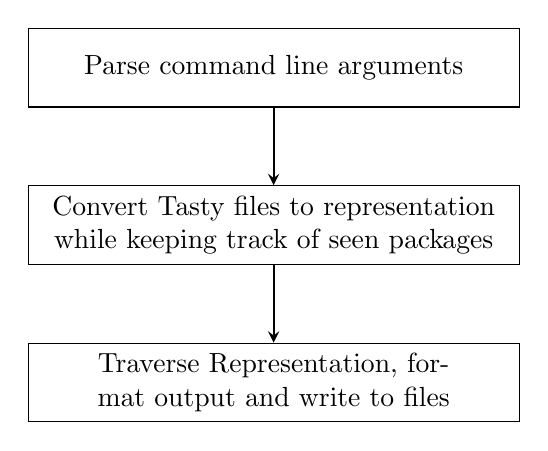
\begin{tikzpicture}[node distance=2cm]
        \node (parse) [process] {Parse command line arguments};
        \node (convert) [process, below of=parse] {Convert Tasty files to representation while keeping track of seen packages};
        \node (output) [process, below of=convert] {Traverse Representation, format output and write to files};
    
        \draw [arrow] (parse) -- (convert);
        \draw [arrow] (convert) -- (output);
    \end{tikzpicture}
\end{center}

\section{Formatting and writing to files}

Useful ?

\section{Use of dotty-doc for parsing}
\label{sec:dotty-docParsing}

Part of dotty-doc code is a parser for user documentation, basically parsing it and also getting every @. Althought the code is more complex than it should, it does the job right and hence is used for this tool. Obviously it needed some adjustements but as we have a very similar structure as Dott-doc's entities, the code nearly worked out of the box when refactoring \texttt{Entity} to \texttt{Representation}.

Note that it is using a library called flexmark-java\footnote{\url{https://github.com/vsch/flexmark-java}} for parsing Markdown.

The parser handles the wiki syntax as well as the Markdown syntax for user documentation.

\chapter{Problems encountered and further work}
\section{Problems encountered}
Here is a listing of a few problems encountered:
\begin{itemize}
    \item All the cons listed in \autoref{sec:proscons}
    \item Multi level list are not parsed correctly when ordered and unordered list are combined, they are parsed as 2 separate list. This is a problem in flexmark-java
    \item If a type (class or type alias) inside a class has the same name as a def/val/var in the same class, for linking to them directly (anchor basically), there is no way to do it in markdown (there is no id, except for title). To counter this problem we list types before values so that it will always jump to the first one
\end{itemize}

\section{Further work}
Further work would include:
\begin{itemize}
    \item Make a library for outputing markdown with escaping. For example, right now, if a method is named \texttt{\#} it will cause a problem
    \item Handle correctly Type Lambdas, right now they are handeled as constant reference
    \item Propose a default HTML/CSS template for people who just want something working out of the box.
    \item Simplify user documentation parsing code taken from Dotty-doc
\end{itemize}

\chapter{Conclusion}

\end{document}

% Expands introduction
% Move flaws into own section
% Avoid bulletpoints
% Architecture
% Reuse of dotty-doc backend thanks to structure
% Explain dotty doc does not do a good job at xxx and result in yyy
% Expands pros and cons of output
% Remove 3.3